\chapter{Background}
\label{sec:background}
\section{Library Dependencies and Migrations}
Being one of the most used programming language, the nodeJS libraries has become one of the most used components in contemporary software development.
The npmJS platform itself hosts the largest collection of user-contributed libraries, which spreads over 700,000 packages that are been downloaded by millions of users on a daily basis. 
Furthermore, the npm ecosystem of packages have been the target of recent studies for researchers \cite{Wittern:2016,Kikas:2017,decan2018impact}.

%expand
Recent events such as the npm leftpad incident \cite{Web:left-pad} and epidemic vulnerabilities such as heartbleed \cite{Web:heartbleed} that have spread throughout an ecosystem have triggered a reaction within the industry.
This is evident by a rise in tool support and security organizations such as \texttt{snyk.io}\footnote{website at \url{https://snyk.io/}} and \texttt{greenkeeper.io}\footnote{website as \url{https://greenkeeper.io/}} gaining more popularity among developers.
For example, it has become common for GitHub projects to display a badge, that socially shows that the project is keeping up to date with its dependencies \cite{Trockman:2018,Mirhosseini:2017}.

However, the recent tool support focus is on detecting if a vulnerable library is listed in a project, assuming that, if the vulnerable library is included in the project, then the project is vulnerable. I believe that this assumption is actually an overestimation.
Recent studies \cite{Hejderup:2018,Ponta:2018} shows that, many projects that do not actually call the affected function are safe from the vulnerability. I refer to these projects as being \textit{clean} (i.e., they do not execute the affecting code in their client applications).
Conversely, I refer to \textit{used} clients as projects that adopt and execute the vulnerability code.
Similarily, Hejderup et al. studied library migrations at the function level, constructing a call graph to understand the true effect of the vulnerability. 
Their study concluded that analysis at this level is indeed problematic due to execution costs needed to construct these graphs.

%Motivating Example
\section{Motivating Example}

WebSocket (i.e., \texttt{ws} package)\footnote{GitHub repository at \url{https://www.npmjs.com/package/ws}} is described as ``a simple to use, blazing fast, and thoroughly tested WebSocket client and server implementation.'' for the nodeJS distribution.
According to the npm website, the library is very popular (with over 3,158,600 downloads and is  depended upon by 3,785 other libraries) within the npm ecosystem.
In 2016, the CWE disclosed a high severity vulnerability (i.e., Denial of Service (DoS)) that affected clients that used this library (i.e.,  \url{https://snyk.io/vuln/npm:ws:20160624}), urging clients to update if they used any \texttt{ws} versions 1.1.0 and lower.
In fact, the issue was so severe, that it was also published as an advisory by the Node Security Platform (i.e., https://nodesecurity.io/advisories/120).

%%%%%%%%%%%%%%%%%%%%%%%%%%%%%%%%%%%%%
\begin{figure*}[th]
\centering
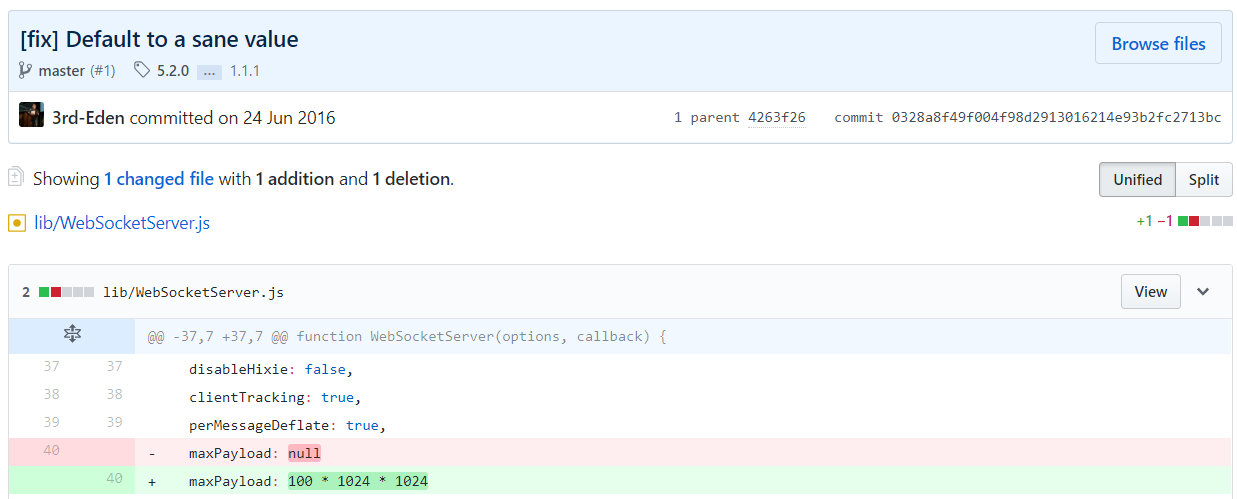
\includegraphics[width=1\textwidth]{images/codeWS.PNG}
\caption{Vulnerability Fix that was applied to the WebSocketServer function in the ws package.}
\label{fig:codeWS}
   \end{figure*}
%%%%%%%%%%%%%%%%%%%%%%%%%%%%%%%%%%%%%

As shown in Figure \ref{fig:codeWS}, the manual inspection of the code reveals that the function \texttt{WebSocketServer} in the file \texttt{WebSocketServer.js} had been modified.
Although small, it does pose as a dependency breaking issue, with client project developer\footnote{the comment is taken from the npm blog at \url{https://github.com/node-red/node-red/issues/931}} stating that \textit{'Indeed, the breaking of node.js 0.10 is precisely why we've not been able to update already'}. 

After consulting the API documentation\footnote{website as \url{https://github.com/websockets/ws/blob/HEAD/doc/ws.md}} and as shown in Figure \ref{fig:codeWSCode}, I find that 
\texttt{WebSocketServer} is not simply a function but is called from the class \textit{WebSocket} which has the \texttt{maxPayload} as one of the option parameters.

%%%%%%%%%%%%%%%%%%%%%%%%%%%%%%%%%%%%%
\begin{figure}[t]
\centering
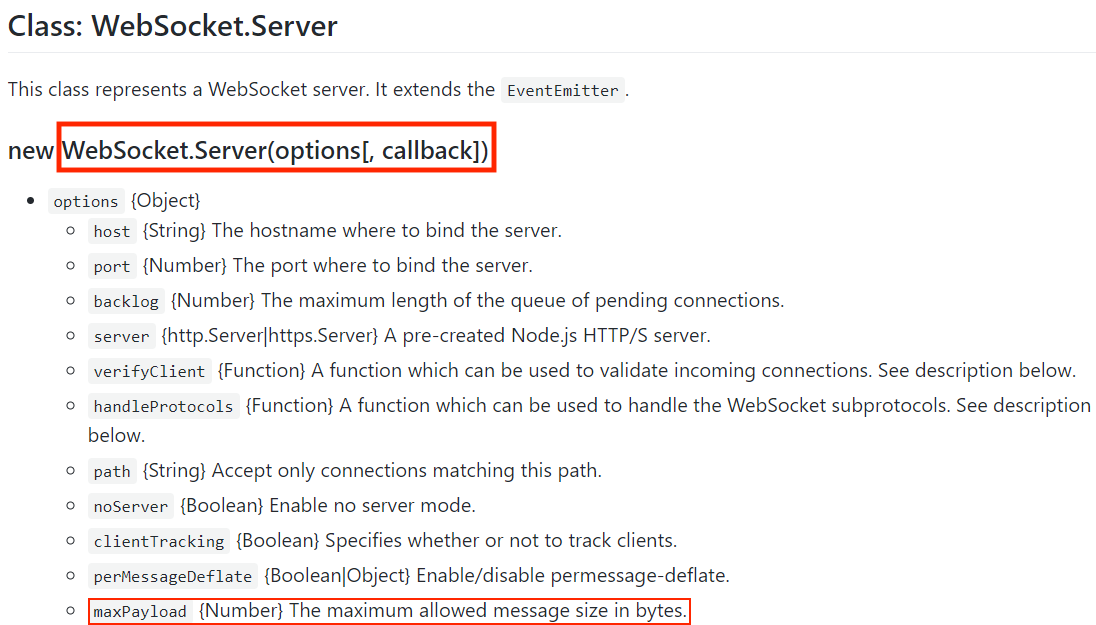
\includegraphics[width=1\textwidth]{images/wcDoc.PNG}
\caption{API documentation for the WebSocket API which is related to the WebSocketServer function.}
\label{fig:codeWSCode}
\end{figure}
%%%%%%%%%%%%%%%%%%%%%%%%%%%%%%%%%%%%%

Furthermore, due to the nature of JavaScript, there can be many different interpretations of the calling function\footnote{A developer blog on the different ways to call a function highlights the variations\url{https://dmitripavlutin.com/6-ways-to-declare-javascript-functions/}}. 
As shown in Listing \ref{code:userhome}, I found at least three ways (i.e., (i) user-defined variable, (ii) call from the \texttt{ws} package and (iii) use the require function) that the client could call the Server function:
\newline
\begin{lstlisting}[language=Java,
caption={Three ways that a client project can call the WebSocketServer function. This is through the WebSocket API.},
label=code:userhome]
    var wss = new WebSocket.Server({ 
    ws.Server({ 
    require('ws').Server; 
\end{lstlisting}

\section{Challenges}
As a result, I find that automation detection is not a trivial task with manual inspection being required to validate the mapping between the affected function and the client-side code in JavaScript.
I summarized the challenges below for JavaScript client projects:

\conclusionbox{
\begin{enumerate}
    \item \textit{Detecting the vulnerable function of the third-party library}. Finding the vulnerable function and trace it to the related public API call, is not trivial.
    \item \textit{Finding the function-calls to a vulnerable third-party library}. Extracting the exposed functions from a project is not a trivial task when manual validation is required.
\end{enumerate}}

Both of the challenges mentioned require a lot of manual validation work. In this thesis I am addressing the 2nd challenge to make the analysis task from vulnerable dependencies an easier task for developers by automating the detection of function-calls. I am focusing on the node.js package manager (npm) repository for JavaScript and therefore I will be defining a third-party library as any set of functions that are available to use in a JavaScript project through an import of an npm package.  
 
Further in this thesis, the terms \textit{Dependencies} and \textit{Libraries} will be used interchangeably always in reference to \textit{third-party libraries}.